\subsection{Joint Distributions}

\subsubsection{Joint, Marginal and Conditional Distributions}
{
			\setlength{\extrarowheight}{3pt}
		
			\begin{twoColTable}
				\hline
				\twoColHdrRow{Discrete Joint Probability Distribution}\\
				\hline
				The \textbf{Joint Probability Distribution} of $X$ and $Y$ is defined by the following distributions:
					& $P(X=x, Y=y)$, $x \in W_x,y \in W_y$\\
				\hline	
				\textbf{Marginal Distributions} are single distributions $P(X=x)$ of $X$ and $P(Y=y)$ of $Y$. They can be calculated based on their joint distribution:
				& $P(X=x)=\sum\limits_{y \in W_y} P(X=x,Y=y)$, $x \in W_x$\\
				Joint distribution of $(X,Y)$ starting from the marginal distribution of $X$ and $Y$ is only possible for \textbf{independent} $X$ and $Y$. Then it holds:
				& $P(X=x, Y=y)=P(X=x) \cdot P(Y=y)$, $x \in W_x,y \in W_y$\\	
				\hline	
				\textbf{Conditional probability} of $X$ given $Y=y$ is defined as:
				& $P(X=x|Y=y)=\frac{P(X=x,Y=y)}{P(Y=y}$\\
				The \textbf{marginal distributions} then can be expressed as follows:
				& $P(X=x)=\sum\limits_{y \in W_y} P(X=x|Y=y)P(Y=y)$, $x \in W_x$\\
				\hline
				\textbf{Conditional Expected Value} of $Y$ given $X=x$ is defined as:
				& $E[Y|X=x]=\sum\limits_{y \in W_y} y \cdot P(Y=y|X=x)$\\	
				\hline
				\hline
				\twoColHdrRow{Example}\\
				\hline
				\vspace*{1cm}
\centering 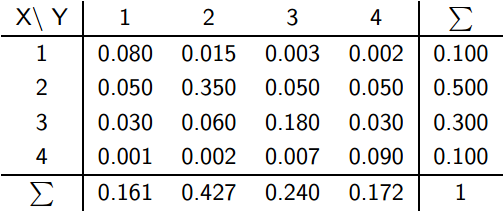
\includegraphics[width=1\linewidth]{images/tableJointDist.png}
				& $P(X=3, Y=4)=0.030$ or $P(X=3 \cup Y=4)=0.030$\vfill
				\vspace*{0.3cm}
				  $P(X=3) = P(X=3, Y=1)+P(X=3, Y=2)+$ \vfill $P(X=3, Y=3)+P(X=3, Y=4) = $\vfill
				  $0.030+0.060+0.180+0.030=0.300$\vfill
				\vspace*{0.3cm}
				$P(Y=2|X=4)=\frac{P(Y=2,X=4)}{P(X=4)}=\frac{0.002}{0.1}=0.02$					\vfill
				\vspace*{0.3cm} 
				$P(X=Y)= P(X=1, Y=1)+P(X=2, Y=2)+$ \vfill $P(X=3, Y=3)+P(X=4, Y=4) = 0.700$\vfill
				\vspace*{0.3cm}
				If random variables are independent it must hold that \vfill
				{$P(X=x, Y=y)=P(X=x) \cdot P(Y=y)$}\vfill
				From the marginal distribution follows \vfill				
				{$P(X=1) \cdot P(Y=2) = 0.100 \cdot 0.427 = 0.043$}			\vfill
				and this is not equal to\vfill
				{$P(X=1, Y=2)= 0.15$}\vfill
				$X$ and $Y$ are \textbf{not independent}\\ 
				\hline
\end{twoColTable}

\begin{twoColTable}
				\hline
				\twoColHdrRow{Joint Density Function}\\
				\hline
				The \textbf{probability} that the \textbf{joint random variable} ($X$,$Y$) lies in a two-dimensional region A, i.e., $A \subset \mathbb{R}^2$, is given by
& $P((X,Y)\in A) = \iint\limits_A f_{X,Y}(x,y)dx\,dy$ \\
The (bivariate) \textbf{joint density function} needs to satisfy& $ \iint\limits_{\mathbb{R}} f_{X,Y}(x,y)dx\,dy = 1$\\
$X$ and $Y$ are only \textbf{independent} if
& $f_{X,Y}(x,y) = f_X(x) \cdot f_Y(y)$, $x,y \in \mathbb{R}$\\
\hline
\textbf{Marginal Density}
& $f_X(x)= \int\limits_{-\infty}^{\infty} f_{X,Y}(x,y) dy$, $f_Y(y)= \int\limits_{-\infty}^{\infty} f_{X,Y}(x,y) dx$\\
\hline
\textbf{Conditional Probability}
& $f_{Y|X=x}(y)=f_Y(y|X=x)=\frac{f_{X,Y}(x,y)}{f_{X}(x)}$\\
$X$ and $Y$ are only independent if the following apply:
&$f_{Y|X=x}(y) = f_Y(y)$ resp. $f_{X|Y=y}(x) = f_X(x)$\\
\hline
\textbf{Conditional Expected Value} of a continuous random variable $Y$ given $X=x$
& $E[Y|X=x]= \int\limits_{-\infty}^{\infty} y \cdot f_{Y|X=x}(y)dy$
\\
\hline
\twoColHdrRow{Example}\\
\hline
Two machines with exponentially distributed life expectancy $X \sim Exp(\lambda_1)$ and $Y \sim Exp(\lambda_2)$, where $X$ and $Y$ are independent. \vfill
$f_X(x) = \lambda_1 e^{-\lambda_1 x}$ and $f_Y(y) = \lambda_2 e^{-\lambda_2 y}$ \vfill
\vspace*{0.3cm}
\centering 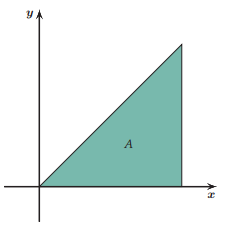
\includegraphics[width=0.5 \linewidth]{images/integrationJointDensityFct.png}
& Due to independence:\vfill
$_{X,Y}(x,y)= \lambda_1 e^{-\lambda_1 x}\lambda_2 e^{-\lambda_2 y}$\vfill
\vspace*{2cm}
$P(Y<X)= \int\limits_0 \limits^{\infty} (\int\limits_0 \limits^{x} \lambda_1 e^{-\lambda_1 x}\lambda_2 e^{-\lambda_2 y} dy)dx$ \vfill
$P(Y<X)= \int\limits_0 \limits^{\infty}  \lambda_1 e^{-\lambda_1 x} (1-e^{-\lambda_2 y})dx = \frac{\lambda_2}{\lambda_1 + \lambda_2}$\\
\hline
\end{twoColTable}
}
\subsubsection{Covariance and Correlation}
{
\setlength{\extrarowheight}{3pt}
		
\begin{twoColTable}
			\hline
			\twoColHdrRow{Covariance and Correlation}\\
			\hline
			\textbf{Covariance}
			& $Cov(X,Y)=E[(X-\mu_X)(Y-\mu_Y)]= E[XY]-E[X]E[Y]$\\
			$X,Y$ independent
			& $E[XY]=E[X]E[Y]$\\
			& $Cov(X,X)=E[(X-\mu_X)(X-\mu_X)] =E[(X-\mu_X)^2] = Var(X) $\\
			Sum of Variances
			& $Var(\sum\limits_{i=1}\limits^{n} X_i)=Cov(\sum\limits_{i=1}\limits^{n} X_i,\sum\limits_{i=1}\limits^{n} X_i)= \sum\limits_{i=1}\limits^{n}Var(X_i)+2\sum\limits_{i<j}\limits^{n} Cov(X_i,X_j)$\\
			2 Random Variables
			& $Var(X+Y)=Cov(X+Y,X+Y)=Var(X)+Var(Y)+2Cov(X,Y)$\\
			If all $X_i$ are independent
			& $Var(X_1 +X_2 +...+X_n)=Var(X_1)+...+Var(X_n)$\\
			\hline
			\textbf{Correlation}
			& $ Cor(X,Y) = \rho_{XY} = \frac{Cov(X,Y}{\rho_X \rho_Y}$ where $-1 \leq Cor(X,Y) \leq 1$\\
			Measure for strength and direction of the \textit{linear dependency} between $X$ and $Y$.
			& $Cor(X,Y)=+1$ if $Y=a+bX$ for $a \in \mathbb{R}$ and $b>0$ \vfill
			$Cor(X,Y)=-1$ if $Y=a+bX$ for $a \in \mathbb{R}$ and $b<0$ 
			\\
			&$|Cor(X,Y)| = 1$ means perfect linear relationship between $X$ and $Y$.\\
			&$Cor(X,Y) = 0$ means $X$ and $Y$ are uncorrelated.\\
			$X$ and $Y$ \textbf{linear independent}
			& $Cor(X,Y) = 0$ (and thus $Cov(X,Y)=0)$\\
			\hline
\end{twoColTable}
		\begin{figure}[H]\centering
			\includegraphics[scale=1]{images/Correlation.png}
			\caption{Correlations}
		\end{figure}
}
\subsubsection{Bivariate Normal Distribution}
{
\begin{twoColTable}
			\hline
			\twoColHdrRow{Bivariate Normal Distribution}\\
			\hline
			Expected values and variances of the marginal distribution
			& $\mu_X, \sigma_X^2$ and $\mu_Y, \sigma_Y^2$\\
			Covariance between $X$ and $Y$
			& $Cov(X,Y)=\rho_{XY}\sigma_X\sigma_Y$\\
			\hline
			Joint Density
			& $f_{X,Y}(x,y)=$\\
			&$\frac{1}{2\pi\sqrt{det(\sum)}}exp\bigg(-\frac{1}{2}(x-\mu_X,y-\mu_Y)\sum^{-1}				\begin{pmatrix}
				x-\mu_X\\
				y-\mu_Y\\
			\end{pmatrix}\bigg)$\\
			\hline
			Covariance Matrix
			& $\sum = \begin{pmatrix}
			Cov(X,X) & Cov(X,Y)\\
			Cov(Y,X) & Cov(Y,Y)\\
			\end{pmatrix}
			= 
			\begin{pmatrix}
			\sigma_X^2 & \rho_{XY}\sigma_X\sigma_Y\\
			\rho_{XY}\sigma_X\sigma_Y & \sigma_Y^2\\
			\end{pmatrix}$\\
			\hline
\end{twoColTable}
}
\subsubsection{Principal Component Analysis (PCA)}
{
PCA is a popular approach for deriving a low-dimensional set of features from a large set of variables. PCA is a technique for reducing the dimension of a $n$ x $p$ data matrix $X$ where $n$ corresponds to the number of observations and $p$ to the number of  variables.
\paragraph{Example: USArrests}
\begin{figure}[H]\centering
\begin{minipage}[c]{0.5\textwidth}
	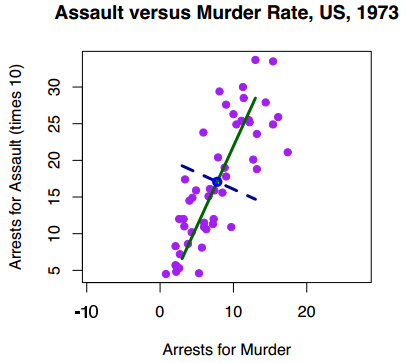
\includegraphics[width=1\linewidth]{images/USArrests_PCA.png}
\end{minipage}\hfill
\begin{minipage}[c]{0.5\textwidth}
	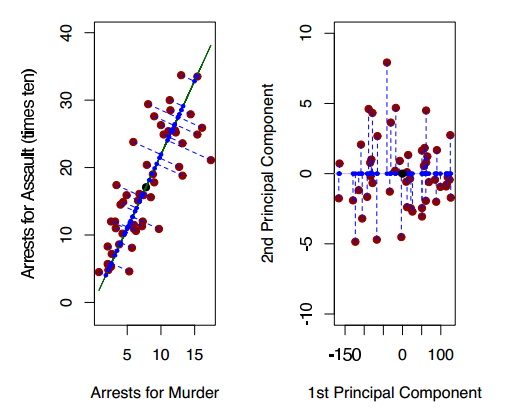
\includegraphics[width=1\linewidth]{images/USArrests_PCA2.png}
\end{minipage}\hfill
\begin{minipage}[t]{.5\textwidth}
	\subcaption{The data vary the most along the first principal component}
\end{minipage}\hfill
\begin{minipage}[t]{.5\textwidth}
	\subcaption{Counter Clockwise Rotation that 1. PC coincides with x-axis}
\end{minipage}
\caption{1st and 2nd Principal Component}
\end{figure}

\begin{figure}[H]\centering
	\begin{minipage}[c]{0.5\textwidth}
		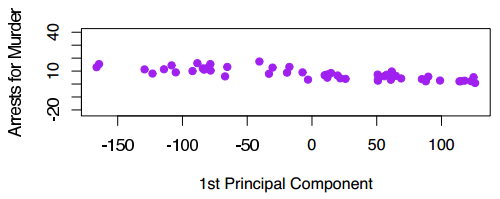
\includegraphics[width=1\linewidth]{images/USArrests_PCA3.png}
	\end{minipage}\hfill
	\begin{minipage}[c]{0.5\textwidth}
		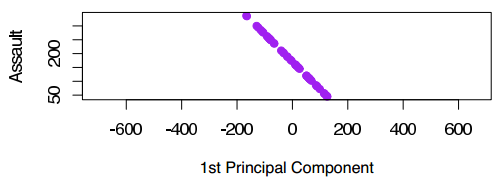
\includegraphics[width=1\linewidth]{images/USArrests_PCA4.png}
	\end{minipage}\hfill
	\begin{minipage}[t]{.5\textwidth}
		\subcaption{$z_{i1}$ versus Murder}
	\end{minipage}\hfill
	\begin{minipage}[t]{.5\textwidth}
		\subcaption{$z_{i1}$ versus Assault}
	\end{minipage}
\end{figure}

\begin{figure}[H]\centering
	\begin{minipage}[c]{0.5\textwidth}
		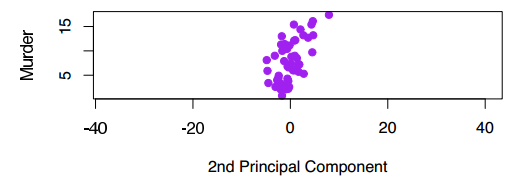
\includegraphics[width=1\linewidth]{images/USArrests_PCA5.png}
	\end{minipage}\hfill
	\begin{minipage}[c]{0.5\textwidth}
		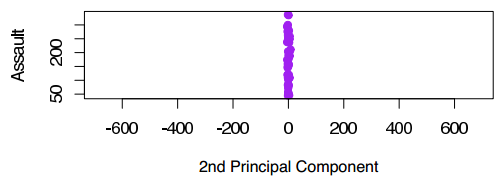
\includegraphics[width=1\linewidth]{images/USArrests_PCA6.png}
	\end{minipage}\hfill
	\begin{minipage}[t]{.5\textwidth}
		\subcaption{$z_{i2}$ versus Murder}
	\end{minipage}\hfill
	\begin{minipage}[t]{.5\textwidth}
		\subcaption{$z_{i2}$ versus Assault}
	\end{minipage}
\caption{The fact that the 2nd principal component scores are much closer to zero indicates that this component captures far less information as the 1st principal component.}
\end{figure}
\RTheory
{	$Z_1=-0.0419126$(Murder - $\overline{\mbox{Murder}})-0.9991213$(Assault-$\overline{\mbox{Assault}})$
	\newline
	\newline
$\phi_{11} = - 0.00419126$ and $\phi_{21} = -0.9991213$ are the \textit{principal component loadings}
\newline
\newline
The idea is that every that out of every linear combination of Murder and Assault sucht that% 
$$\phi_{11}^2+\phi_{21}^2 = 1$$
and \vfill
$$Var(\phi_{11})(\mbox{Murder}-\overline{\mbox{Murder}})+\phi_{21}(\mbox{Assault}-\overline{\mbox{Assault}})$$
is maximized. 
\newline
\newline
{\color{blue}prcomp()} centers the variables to have mean zero. This corresponds to how the first principal component is defined.
\newline
\newline
$z_{i1}=-0.0419126$(Murder - $\overline{\mbox{Murder}})-0.9991213$(Assault-$\overline{\mbox{Assault}})$
\newline
\newline
The values of $z_{i1},...,z_{n1}$ are known as \textit{principal component scores}, seen in the right-hand panel in Figure 6. $z_{i1} > 0$ indicates a state with below-average arrests for murder and below average for assault. A negative score suggests the opposite.
\newline
\newline
	$Z_2=0.9991213$(Murder - $\overline{\mbox{Murder}})-0.0419126$(Assault-$\overline{\mbox{Assault}})$
 }
	{sections/ProbabilityStatistics/JointDistributions/RCode/USArrests_prcomp.R}

	With two-dimensional data, such as in our USArrests example, we can construct at most two principal components. However, if we had other variables, such as Rape, then additional components could be constructed.
	
	\paragraph{PCA and Covariance Matrix}
	{The covariance matrix of two random variables $X$ and $Y$ is defined as 
		$$\sum = 
		\begin{pmatrix}
		Cov(X,X) & Cov(X,Y) \\
		Cov(Y,X) & Cov(Y,Y) \\
		\end{pmatrix}
		=
		\begin{pmatrix}
		\sigma_X^2 & Cov(X,Y) \\
		Cov(Y,X) & \sigma_Y^2 \\
		\end{pmatrix}
	 $$	
	Since $Z_1$ and $Z_2$ are required to be uncorrelated, this implies for their covariance matrix $\sum$ to have vanishing off diagonal elements. Therefore the covariance has to be diagonalized. This can be done with by a rotation matrix $\Phi$ so that
	$$ 
	\begin{pmatrix}
	Z_1\\
	Z_2\\
	\end{pmatrix}
	 = (X-\mu_X,Y-\mu_Y)
	 \begin{pmatrix}
	 \phi_{11}&\phi_{12}\\
	 \phi_{21}&\phi_{22}\\
	 \end{pmatrix}
	 =
	 \begin{pmatrix}
	 \phi_{11}(X-\mu_X)&\phi_{12}(Y-\mu_Y)\\
	 \phi_{21}(X-\mu_X)&\phi_{22}(Y-\mu_Y)\\
	 \end{pmatrix}
	 $$
	 and
	 $$
	 \begin{pmatrix}
	 Cov(Z_1,Z_1)&Cov(Z_1,Z_2)\\
	 Cov(Z_2,Z_1)&Cov(Z_2,Z_2)\\
	 \end{pmatrix}
	 =
	 \begin{pmatrix}
	 	\sigma_{Z_1}^2&0\\
	 	0&\sigma_{Z_2}^2\\
	 \end{pmatrix}
	 $$
	 The rotation matrix $\Phi$ needs to satisfy the condition $\phi_{11}^2+ \phi_{21}^2=1$ and $\phi_{12}^2+\phi_{22}^2=1$
	 It is straightforward to generalize the case of $p=2$ to an arbitrary $p$. 
	}
	\paragraph{Proportion of Variance Explained by Principal Components}
	\RTheory
	{
	There is an information loss of the given data by projecting the observations onto the first few principal components. Therefore we want to know the \textit{proportion of variance explained (PVE)}. The \textit{total variance} is defined as
	$$
	\sum\limits_{j=1}\limits^{p} Var(X_j)=\sum\limits_{j=1}\limits^{p}\frac{1}{n}\sum\limits_{i=1}\limits^{n}x_{ij}^2
	$$	
	and the variance of the $m$th principal component is
	$$
	\frac{1}{n}\sum\limits_{i=1}\limits^{n}z_{im}^2=\frac{1}{n}\sum\limits_{i=1}\limits^{n}\bigg(\sum\limits_{j=1}\limits^{p}\phi_{jm}x_{ij}\bigg)^2
	$$
	Therefore the PVE by the $m$th principal component is given by
	$$
\frac{\sum\limits_{i=1}\limits^{n}\bigg(\sum\limits_{j=1}\limits^{p}\phi_{jm}x_{ij}\bigg)^2}{\sum\limits_{j=1}\limits^{p}\sum\limits_{i=1}\limits^{n}x_{ij}^2}
	$$
	}
	{sections/ProbabilityStatistics/JointDistributions/RCode/USArrests_pve.R}

	


}
